\subsection{Traffic Demand Per Subscriber}\label{subsec:behavior}

\begin{figure}[t]
\begin{minipage}{1\linewidth}
\centering
%
\begin{subfigure}[b]{.99\linewidth}
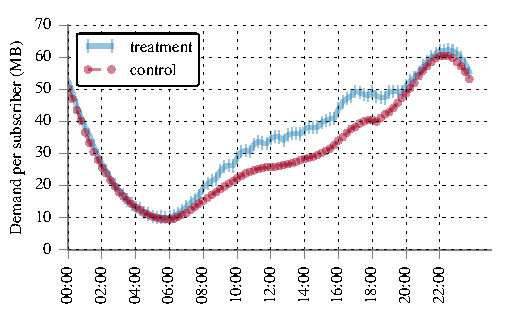
\includegraphics[width=\linewidth]{figures/weekday_demand_mean.pdf}
               \caption{Weekday traffic demand\label{fig:weekday-daily-usage}}
\end{subfigure}
%
\begin{subfigure}[b]{.99\linewidth}
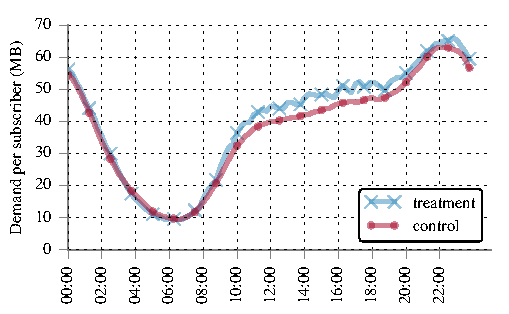
\includegraphics[width=\linewidth]{figures/weekend_demand_mean.pdf}
               \caption{Weekend traffic demand\label{fig:weekend-daily-usage}}
\end{subfigure}
%
\end{minipage}
\caption{Average subscriber demand (bytes every 15-minutes)}
\label{fig:traffic-demand-timeseries}
\end{figure}

Figure \ref{fig:traffic-demand-timeseries} shows the downlink traffic demand (bytes)
of an average subscriber over a 15-minute measurement period in a week.
We observe that subscriber behavior differs
significantly on weekdays and weekends. On weekdays, traffic demand 
increases monotonically from morning until prime-time in the evening. On 
weekends, there is a sharp rise in demand in the early morning period. Then, the
demand plateaus until the next sharp rise during the evening prime-time hours.
Previous reports indicate that the aggregate traffic volume for US fixed access
link providers usually troughs during mid-afternoon hours (between 2:00 PM -- 6:00 PM)
~\cite{sandvine20141h}. We do not observe such a trough in the subscriber 
demand in our dataset.

\begin{figure}[t]
\begin{minipage}{1\linewidth}
\centering
%
\begin{subfigure}[b]{1\linewidth}
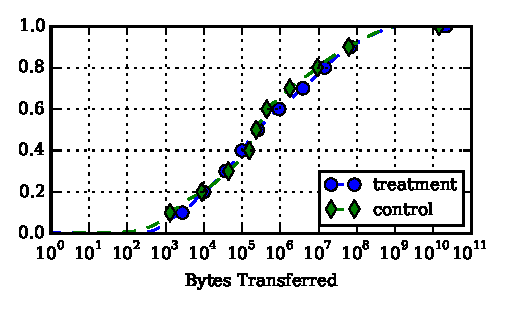
\includegraphics[width=\linewidth]{figures/cdf-all-bytes.pdf}
               \caption{Overall traffic demand for all subscribers at all times\label{fig:CDF-data-rate}}
\end{subfigure}
% maybe should be mean per day?
%
\begin{subfigure}[b]{1\linewidth}
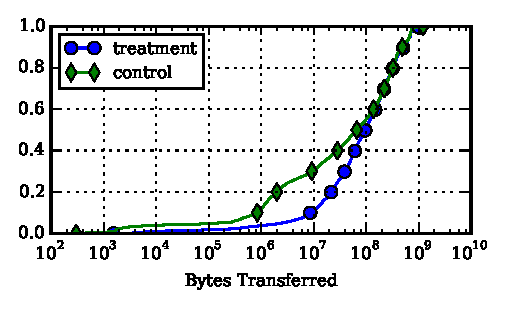
\includegraphics[width=\linewidth]{figures/cdf-per-device-perc95.pdf}
               \caption{Peak (95\%) traffic demand per subscriber\label{fig:CDF-data-rate-perc95}}
\end{subfigure}
%
\end{minipage}
\caption{Traffic demand (bytes every 15-minutes) for \control{} and \treatment{}\label{fig:traffic-demand-cdf}}
\end{figure}

Figure \ref{fig:CDF-data-rate} shows the distribution of the
all bytes transferred in the \treatment{} and \control{} set
over the three months of the dataset. Figure \ref{fig:CDF-data-rate-perc95}
plots the distribution of the peak (95th percentile) demand of the
subscriber over the three months of the dataset. The highest peak
demand achieved by subscribers in the \control{} and \treatment{}
groups were 10 GB in 15-mins. The median peak demand was 80 MB and
100 MB respectively.

We observe that although the overall series are similar, the peak demand of subscribers
is higher in the \treatment{} set. We expected the largest difference
in demands would be in the subscribers who have the heaviest demand already.
But unexpectedly, the lowest demanding 50\% of the subscribers in
\treatment{} have a much higher demand than the lowest demanding 50\% of \control{}.
We confirm that the both groups have similar median demands over each day. However
the daily peak demand is higher for the lowest demanding subscribers in
 \treatment{}, as compared to the lowest demanding subscribers in \control{}.

\begin{figure}[t]
\centering
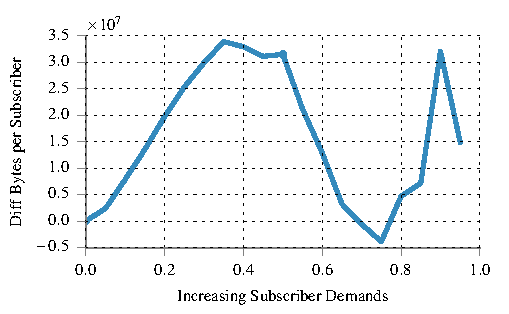
\includegraphics[width=\linewidth]{figures/diff_perc95_bytes_subsc-overall.pdf}
               \caption{Difference between \treatment{} and \control{}
               in peak (95\%) traffic demand\label{fig:diff-perc95}}
\end{figure}

We plot the distribution of the difference in peak subscriber demands for
the lowest to highest demanding subscribers in both groups (Figure~\ref{fig:diff-perc95}).
We see that the peak demand for the lowest demanding 70\% of the households of
the \treatment{} group is higher than the peak demand of the lowest demanding bottom-most
70\% of the \control{} group. These subscribers have a peak demand less than 200 MB.
For 20\% of the subscribers in the \control{} group with peak demands between 10 -- 70 MB,
the equivalent 20\% of the \treatment{} group has peak demands increased by 30 MB.

Under 15\% of subscribers in the \treatment{} group with peak demands more than 200 MB 
peak demands similar, or lower than the equivalent 15\% of subscribers in the \control{}
group, that has a lower capacity. The highest demanding subscribers in the \treatment{}
(beyond 800 MB peak demand) have demands 15 -- 30 MB more than the equivalent 15\% of 
the \control{} group. In contrast, for the upstream, the \treatment{} group consistently has
a 2 MB higher peak traffic demand every 15 minutes as compared to the \control{} group
(except for the top 10\% users in the \treatment{} set who had a higher peak).

On investigating further, we observed that subscribers with low demand traffic 
increased their demand daily by comparable amounts.

There is negligible change in the daily peak 
demand for users who have high demands, and a large increase for users with a low demand.
Furthermore, we observe this affect is also present in the uplink.
There could be many reasons for this increase in demand, such as short
term activities (short videos or web browsing) 
that have a slightly higher traffic demand. Studying the applications 
responsible for such behavioral changes in traffic demand is out of the
scope of this paper and we leave it to future work.